% File: cjupiter-xform.tex

\documentclass{standalone}

\usepackage{tikz}
\usetikzlibrary{shapes, positioning, arrows.meta}

% default horizontal/vertical distance
\def\hdist{1.8}
\def\vdist{1.8}

\newcommand{\state}[2]{% #1: state label; #2: position
  \node (#1) [circle, inner sep = 0pt, minimum size = 6mm, text width = 8mm, align = center, draw, #2, font = \Large] {$#1$};
}

\newcommand{\trans}[4]{
  \draw[>=Stealth, ->] (#1) to node[sloped, #4] {$#3$} (#2);
}

\begin{document}
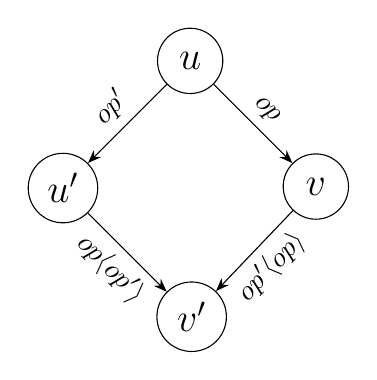
\begin{tikzpicture}[trans/.style = {>=Stealth, ->}]
  \state{u}{}
  \state{u'}{below left = of u}
  \state{v}{below right = of u}
  \state{v'}{below right = of u'}

  \trans{u}{u'}{op'}{above}
  \trans{u}{v}{op}{above}
  \trans{u'}{v'}{op\langle op' \rangle}{below}
  \trans{v}{v'}{op'\langle op \rangle}{below}
\end{tikzpicture}
\end{document}
